\chapter{技术文章与讨论}
\label{chap:3}

该作业其专案为 kancheng/kan-cs-report-in-2021 ,程式码则可于 kan-cs-report-in-2021/AI/pytorch-transformer/code 找到,实验设备为 MacBook Pro (Retina, 15-inch, Mid 2014) 和 Acer Aspire R7。同时参考的技术文章与论文连结皆于该专案的 init.md 文件中条列呈现。该专案根据 Harvard NLP 的 The Annotated Transformer 与名为 fawazsammani/chatbot-transformer 的 GitHub 专案,该专案使用 Cornell Movie Dialog Corpus 资料,进行 Chatbot using Transformers 的实作。作业结果为前者为 transformer-harvard-demo.ipynb ,而后者为 transformer-chatbot-demo.ipynb 档案。

在处理过程中大多遇到 Pytorch 套件不相容、版本过旧的问题,这类问题来源大多是 Pytorch 早期开发功能变动所造成,但可以从 Harvard NLP 与 Chatbot using Transformers 的过程中看出整个 Transformer 的设计概念与运作,程式码的版本进行查错与修正后执行,而两个范例的 Epoch 等训练结果,也于该章进行说明。

\section{技术文章}

在此本章将近期所搜集跟阅读的技术文章与资源进行条列与整理后做表如下所示 :

\subsection{编程}

\begin{center}
\begin{tabular}{cccc}
\hline
主题节录 & 用途 & 分类 & 备注  \\
\hline
tensorflow/tensor2tensor \cite{githubtfws} & 技术 & 编程 & TensorFlow \\
paperswithcode - Attention Is All You Need \cite{pwcws} & 技术 & 编程 & 專案索引 \\
tensorflow/models \cite{githubtfmdws} & 技术 & 编程 & TensorFlow \\
graykode/nlp-tutorial \cite{graykodemdws} & 技术 & 编程 & NLP \\
SamLynnEvans/Transformer \cite{sletferws} & 技术 & 编程 &  \\
huggingface/transformers \cite{huggingfacemdws} & 技术 & 编程 &  \\
harvardnlp/annotated-transformer \cite{harvardnlpatf} & 技术 & 编程 &  \\
fawazsammani/chatbot-transformer \cite{fawazsammanitf17} & 技术 & 编程 &  \\
\hline
\end{tabular}
\end{center}

\subsection{文献说明与综述整理}

\begin{center}
\begin{tabular}{cccc}
\hline
主题节录 & 用途 & 分类 & 备注  \\
\hline
Attention is all you need \cite{vaswani2017attention} & 论文 & 文献 & 最早的文獻 \\
On the Integration of Self-Attention and Convolution \cite{pan2021integration} & 论文 & 文献 &  \\
视觉 Transformer 综述 \cite{zhihutf23} & 技术 & 文献整理 & 综述 \\
Transformer 最新综述 \cite{jackcui24} & 技术 & 文献整理 & 综述 \\
Self-Attention 和 CNN 的优雅集成 \cite{mpweixinqq24} & 技术 & 文献说明 & 研究 \\
\hline
\end{tabular}
\end{center}

\subsection{技术文件与实现}

\begin{center}
\begin{tabular}{cccc}
\hline
主题节录 & 用途 & 分类 & 备注  \\
\hline
搞懂 Transformer 结构 \cite{zhihuscir} & 技术 & 文件 & PyTorch \\
How to code The Transformer in Pytorch \cite{tfmrsle} & 技术 & 文件 & PyTorch \\
The Annotated Transformer \cite{opennmt} & 技术 & 文件 & harvardnlp \\
从零实现了 Transformer 模型 \cite{zhihutf10} & 技术 & 文件 &  \\
This post is all you need \cite{zhihutf11} & 技术 & 文件 &  \\
【機器學習2021】 Transformer (上) \cite{hyltfr12} & 技术 & 影片 &  \\
【機器學習2021】 Transformer (下) \cite{hyltfr13} & 技术 & 影片 &  \\
Transformer Implementation \cite{deepaksaini16} & 技术 & 文件 &  \\
Transformer 的 PyTorch 实现 \cite{deeplnewer18} & 技术 & 文件 &  \\
搞懂 Transformer 结构 \cite{zhihutf19} & 技术 & 文件 &  \\
超详细图解 Self-Attention \cite{zhihutf20} & 技术 & 文件 &  \\
Transformer \cite{zhihutf21} & 技术 & 文件 &  \\
Transformer 详解 \cite{deeplnewer26} & 技术 & 文件 &  \\
\hline
\end{tabular}
\end{center}


\section{程式码与注解说明}

该小节分为两大部分,其一为 Harvard NLP 的成果,前半段根据本作业已经修正的 Pytorch 版本,后续未成功的部分则根据原本的 Harvard NLP,其二为 Chatbot Transformer 的训练。另外 Harvard NLP 的成果与原本的 Transformer 文献架构可以互相呼应并可以当做该论文的补充说明。

\subsection{Harvard NLP}

虽然 "Attention is All You Need" \footnote{https://arxiv.org/abs/1706.03762} 一文中提出的 Transformer 网络结构最近引起了很多人的关注。Transformer 不仅能够明显地提升翻译质量,还为许多 NLP 任务提供了新的结构。虽然原文写得很清楚,但实际上大家普遍反映很难正确地实现 Transformer。

所以我们为此文章写了篇注解文档,并给出了一行行实现的 Transformer 的代码。本文档删除了原文的一些章节并进行了重新排序,并在整个文章中加入了相应的注解。此外,本文档以 Jupyter notebook 的形式完成,本身就是直接可以运行的代码实现,总共有 400 行库代码,在 4 个 GPU 上每秒可以处理 27,000 个 tokens。

想要运行此工作,首先需要安装 PyTorch\footnote{https://pytorch.org/}。这篇文档完整的 notebook 文件及依赖可在 GitHub\footnote{https://github.com/harvardnlp/annotated-transformer} 或 Google Colab\footnote{https://drive.google.com/file/d/1xQXSv6mtAOLXxEMi8RvaW8TW-7bvYBDF/view?usp=sharing} 上找到。需要注意的是,此注解文档和代码仅作为研究人员和开发者的入门版教程。这里提供的代码主要依赖 OpenNMT \footnote{https://opennmt.net/} 进行实现,想了解更多关于此模型的其他实现版本可以查看 Tensor2Tensor\footnote{https://github.com/tensorflow/tensor2tensor} (tensorflow 版本) 和 Sockeye\footnote{https://github.com/awslabs/sockeye} (mxnet版本)

Alexander Rush (@harvardnlp\footnote{https://twitter.com/harvardnlp} or srush@seas.harvard.edu)

\begin{figure}[htb]
\centering 
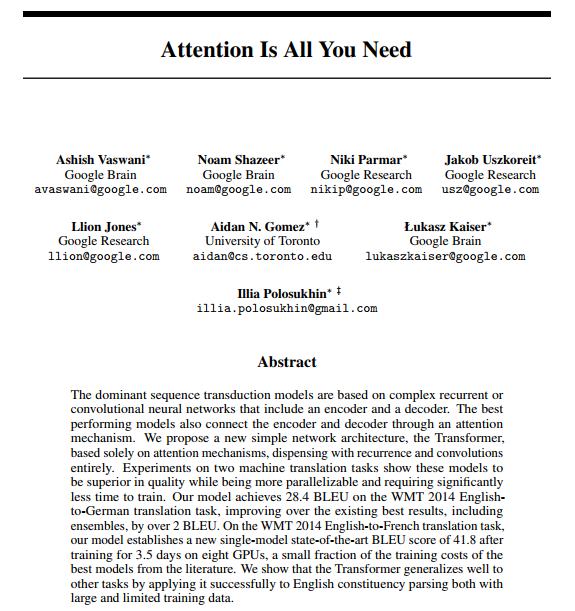
\includegraphics[width=0.8\textwidth]{img/n0.png} 
\caption{Attention is All You Need}
\label{Test}
\end{figure}

0. 准备工作 (Prelims)

\begin{Verbatim}
# http://download.pytorch.org/whl/cu80/torch-0.3.0.post4
# 该版本过于老旧

# http://nlp.seas.harvard.edu/2018/04/03/attention.html
import numpy as np
import torch
import torch.nn as nn
import torch.nn.functional as F
import math, copy, time
from torch.autograd import Variable
import matplotlib.pyplot as plt
import seaborn
seaborn.set_context(context="talk")
%matplotlib inline
print(torch.__version__)
\end{Verbatim}

\begin{figure}[htb]
\centering 
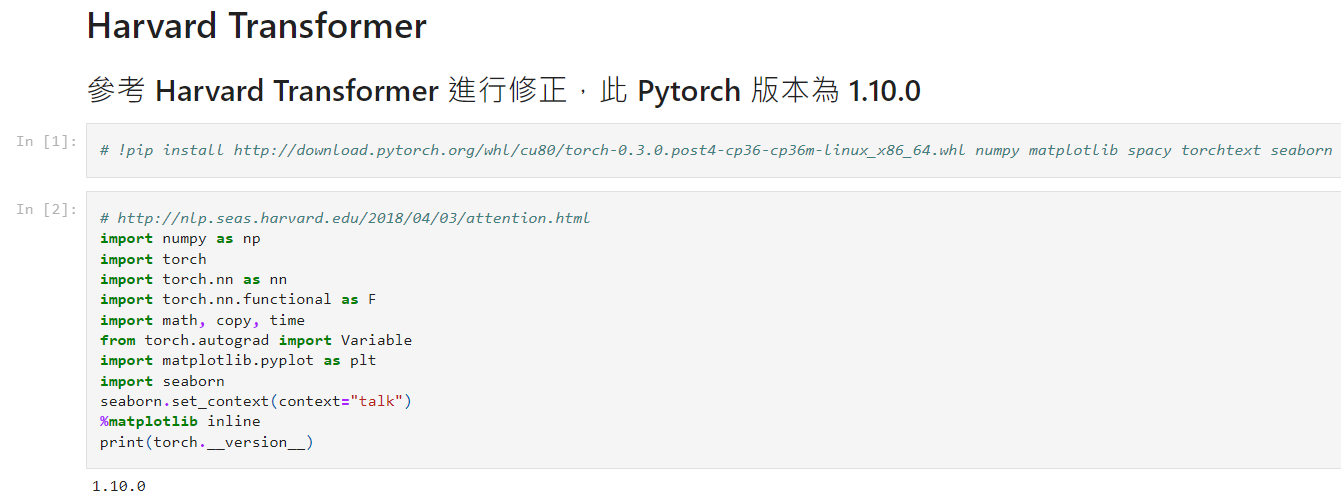
\includegraphics[width=0.95\textwidth]{img/nn0.png} 
\caption{作業版本 Pytorch 修正}
\label{Test}
\end{figure}

内容目录 (Table of Contents)

\begin{itemize}
\item [-] 准备工作 (Prelims)
\item [-] 背景 (Background)
\item [-] 模型结构 (Model Architecture)
\begin{itemize}
\item [-] Encoder 和 Decoder (Encoder and Decoder Stacks)
\begin{itemize}
\item [-] Encoder
\item [-] Decoder
\item [-] Attention
\item [-] Attention 在模型中的应用 (Applications of Attention in our Model)
\end{itemize}
\item [-] Position-wise 前馈网络 (Position-wise Feed-Forward Networks)
\item [-] Embedding 和 Softmax (Embeddings and Softmax)
\item [-] 位置编码 (Positional Encoding)
\item [-] 完整模型 (Full Model)
\end{itemize}
\item [-] 训练 (Training)
\begin{itemize}
\item [-] 批和掩码 (Batches and Masking)
\item [-] 训练循环 (Training Loop)
\item [-] 训练数据和批处理 (Training Data and Batching)
\item [-] 硬件和训练进度 (Hardware and Schedule)
\item [-] 优化器 (Optimizer)
\item [-] 正则化 (Regularization)
\item [-] 标签平滑 (Label Smoothing)
\end{itemize}
\item [-] 第一个例子 (A First Example)
\begin{itemize}
\item [-] 数据生成 (Synthetic Data)
\item [-] 损失计算 (Loss Computation)
\item [-] 贪心解码 (Greedy Decoding)
\end{itemize}
\item [-] 真实示例 (A Real World Example)
\begin{itemize}
\item [-] 数据加载 (Data Loading)
\item [-] 迭代器 (Iterators)
\item [-] 多 GPU 训练 (Multi-GPU Training)
\item [-] 训练系统 (Training the System)
\item [-] 附加组件:BPE,搜索,平均 (Additional Components: BPE, Search, Averaging)
\end{itemize}
\item [-] 结果 (Results)
\begin{itemize}
\item [-] 注意力可视化 (Attention Visualization)
\end{itemize}
\item [-] 结论 (Conclusion)
\end{itemize}

1. 背景 (Background)

减少序列处理任务的计算量是一个很重要的问题,也是 Extended Neural GPU、ByteNet和ConvS2S 等网络的动机。上面提到的这些网络都是以  CNN 为基础,并行计算所有输入和输出位置的隐藏表示。

在这些模型中,关联来自两个任意输入或输出位置的信号所需的操作数随位置间的距离增长而增长,例如 ConvS2S 呈线性增长,ByteNet 呈现以对数形式增长,这会使学习较远距离的两个位置之间的依赖关系变得更加困难。而在Transformer中,其操作次数则被减少到了常数级别。

Self-attention 有时候也被称为 Intra-attention,是在单个句子不同位置上做的 Attention,并得到序列的一个表示。它能够很好地应用到很多任务中,包括阅读理解、摘要、文本蕴涵,以及独立于任务的句子表示。端到端的网络一般都是基于循环注意力机制而不是序列对齐循环,并且已经有证据表明在简单语言问答和语言建模任务上表现很好。

据我们所了解,Transformer 是第一个完全依靠 Self-attention 而非使用序列对齐的RNN或卷积的方式来计算输入输出表示的转换模型。

2. 模型结构 (Model Architecture)

目前大部分比较热门的神经序列转换模型都有 Encoder-Decoder 结构\footnote{https://arxiv.org/abs/1409.0473}。Encoder将输入序列 $(x_1, ..., x_n) $ 映射到一个连续表示序列 $z = (z_1, ..., z_n) $。

对于编码得到的z,Decoder每次解码生成一个符号,直到生成完整的输出序列:$(y_1, ..., y_m)$ 。对于每一步解码,模型都是自回归的\footnote{https://arxiv.org/abs/1308.0850},即在生成下一个符号时将先前生成的符号作为附加输入。

\begin{Verbatim}
class EncoderDecoder(nn.Module):
    """
    A standard Encoder-Decoder architecture. Base for this and many 
    other models.
    """
    def __init__(self, encoder, decoder, src_embed, tgt_embed, generator):
        super(EncoderDecoder, self).__init__()
        self.encoder = encoder
        self.decoder = decoder
        self.src_embed = src_embed
        self.tgt_embed = tgt_embed
        self.generator = generator
        
    def forward(self, src, tgt, src_mask, tgt_mask):
        "Take in and process masked src and target sequences."
        return self.decode(self.encode(src, src_mask), src_mask,
                            tgt, tgt_mask)
    
    def encode(self, src, src_mask):
        return self.encoder(self.src_embed(src), src_mask)
    
    def decode(self, memory, src_mask, tgt, tgt_mask):
        return self.decoder(self.tgt_embed(tgt), memory, src_mask, tgt_mask)
\end{Verbatim}

\begin{Verbatim}
class Generator(nn.Module):
    "Define standard linear + softmax generation step."
    def __init__(self, d_model, vocab):
        super(Generator, self).__init__()
        self.proj = nn.Linear(d_model, vocab)

    def forward(self, x):
        return F.log_softmax(self.proj(x), dim=-1)
\end{Verbatim}

Transformer 的整体结构如下图所示,在 Encoder 和 Decoder 中都使用了 Self-attention, Point-wise 和全连接层。Encoder 和 decoder 的大致结构分别如下图的左半部分和右半部分所示。

3. Encoder 和 Decoder (Encoder and Decoder Stacks)

\begin{figure}[htb]
\centering 
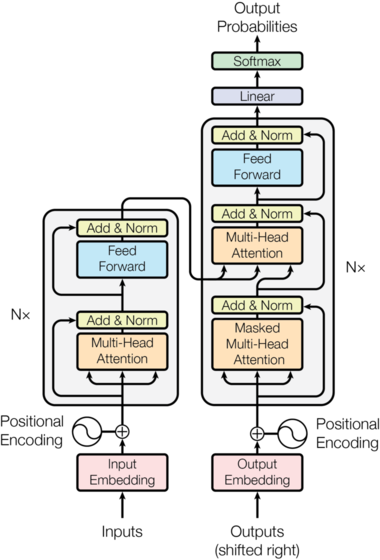
\includegraphics[width=0.5\textwidth]{img/n1.png} 
\caption{Transformer 的整体结构}
\label{Test}
\end{figure}

4. Encoder

Encoder 由 $N = 6$ 个相同的层组成。

%\begin{Verbatim}
%\end{Verbatim}

\begin{Verbatim}
def clones(module, N):
    "Produce N identical layers."
    return nn.ModuleList([copy.deepcopy(module) for _ in range(N)])
\end{Verbatim}

\begin{Verbatim}
class Encoder(nn.Module):
    "Core encoder is a stack of N layers"
    def __init__(self, layer, N):
        super(Encoder, self).__init__()
        self.layers = clones(layer, N)
        self.norm = LayerNorm(layer.size)
        
    def forward(self, x, mask):
        "Pass the input (and mask) through each layer in turn."
        for layer in self.layers:
            x = layer(x, mask)
        return self.norm(x)
\end{Verbatim}

我们在每两个子层之间都使用了残差连接(Residual Connection) \footnote{https://arxiv.org/abs/1512.03385} 和归一化 (layer normalization) \footnote{https://arxiv.org/abs/1607.06450}。

\begin{Verbatim}
class LayerNorm(nn.Module):
    "Construct a layernorm module (See citation for details)."
    def __init__(self, features, eps=1e-6):
        super(LayerNorm, self).__init__()
        self.a_2 = nn.Parameter(torch.ones(features))
        self.b_2 = nn.Parameter(torch.zeros(features))
        self.eps = eps

    def forward(self, x):
        mean = x.mean(-1, keepdim=True)
        std = x.std(-1, keepdim=True)
        return self.a_2 * (x - mean) / (std + self.eps) + self.b_2
\end{Verbatim}

也就是说,每个子层的输出为 $LayerNorm(x + Sublayer(x))$ ,其中 $Sublayer(x)$ 是由子层自动实现的函数。我们在每个子层的输出上使用 Dropout\footnote{https://jmlr.org/papers/v15/srivastava14a.html},然后将其添加到下一子层的输入并进行归一化。

为了能方便地使用这些残差连接,模型中所有的子层和Embedding层的输出都设定成了相同的维度,即 $d_{model} = 512$。

\begin{Verbatim}
class SublayerConnection(nn.Module):
    """
    A residual connection followed by a layer norm.
    Note for code simplicity the norm is first as opposed to last.
    """
    def __init__(self, size, dropout):
        super(SublayerConnection, self).__init__()
        self.norm = LayerNorm(size)
        self.dropout = nn.Dropout(dropout)

    def forward(self, x, sublayer):
        "Apply residual connection to any sublayer with the same size."
        return x + self.dropout(sublayer(self.norm(x)))
\end{Verbatim}

每层都有两个子层组成。第一个子层实现了“多头”的 Self-attention,第二个子层则是一个简单的 Position-wise 的全连接前馈网络。

\begin{Verbatim}
class EncoderLayer(nn.Module):
    "Encoder is made up of self-attn and feed forward (defined below)"
    def __init__(self, size, self_attn, feed_forward, dropout):
        super(EncoderLayer, self).__init__()
        self.self_attn = self_attn
        self.feed_forward = feed_forward
        self.sublayer = clones(SublayerConnection(size, dropout), 2)
        self.size = size

    def forward(self, x, mask):
        "Follow Figure 1 (left) for connections."
        x = self.sublayer[0](x, lambda x: self.self_attn(x, x, x, mask))
        return self.sublayer[1](x, self.feed_forward)
\end{Verbatim}

5. Decoder

Decoder 也是由 $N = 6$ 个相同层组成。

\begin{Verbatim}
class Decoder(nn.Module):
    "Generic N layer decoder with masking."
    def __init__(self, layer, N):
        super(Decoder, self).__init__()
        self.layers = clones(layer, N)
        self.norm = LayerNorm(layer.size)
        
    def forward(self, x, memory, src_mask, tgt_mask):
        for layer in self.layers:
            x = layer(x, memory, src_mask, tgt_mask)
        return self.norm(x)
\end{Verbatim}

除了每个编码器层中的两个子层之外,解码器还插入了第三种子层对编码器栈的输出实行“多头”的 Attention。与编码器类似,我们在每个子层两端使用残差连接进行短路,然后进行层的规范化处理。

\begin{Verbatim}
class DecoderLayer(nn.Module):
    "Decoder is made of self-attn, src-attn, and feed forward (defined below)"
    def __init__(self, size, self_attn, src_attn, feed_forward, dropout):
        super(DecoderLayer, self).__init__()
        self.size = size
        self.self_attn = self_attn
        self.src_attn = src_attn
        self.feed_forward = feed_forward
        self.sublayer = clones(SublayerConnection(size, dropout), 3)
 
    def forward(self, x, memory, src_mask, tgt_mask):
        "Follow Figure 1 (right) for connections."
        m = memory
        x = self.sublayer[0](x, lambda x: self.self_attn(x, x, x, tgt_mask))
        x = self.sublayer[1](x, lambda x: self.src_attn(x, m, m, src_mask))
        return self.sublayer[2](x, self.feed_forward)
\end{Verbatim}

我们还修改解码器中的 Self-attention 子层以防止当前位置 Attend 到后续位置。这种 Masked 的 Attention 是考虑到输出 Embedding 会偏移一个位置,确保了生成位置 $i$ 的预测时,仅依赖小于 $i$ 的位置处的已知输出,相当于把后面不该看到的信息屏蔽掉。

\begin{Verbatim}
def subsequent_mask(size):
    "Mask out subsequent positions."
    attn_shape = (1, size, size)
    subsequent_mask = np.triu(np.ones(attn_shape), k=1).astype('uint8')
    return torch.from_numpy(subsequent_mask) == 0
\end{Verbatim}

下面的 Attention mask 图显示了允许每个目标词(行)查看的位置(列)。在训练期间,当前解码位置的词不能 Attend 到后续位置的词。

\begin{Verbatim}
plt.figure(figsize=(5,5))
plt.imshow(subsequent_mask(20)[0])
None
\end{Verbatim}

\begin{figure}[htb]
\centering 
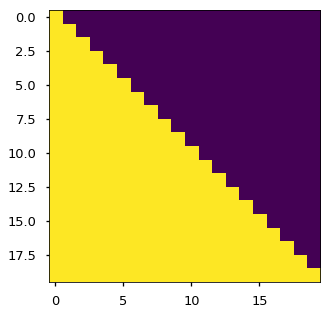
\includegraphics[width=0.5\textwidth]{img/n2.png} 
\caption{Attention mask 图}
\label{Test}
\end{figure}

6. Attention

Attention 函数可以将 Query 和一组 Key-Value 对映射到输出,其中 Query、Key、Value 和输出都是向量。 输出是值的加权和,其中分配给每个 Value 的权重由 Query 与相应 Key 的兼容函数计算。

我们称这种特殊的 Attention 机制为 "Scaled Dot-Product Attention"。输入包含维度为 $d_{k}$ 的 Query 和 Key,以及维度为 $d_v$ 的Value。 我们首先分别计算 Query 与各个 Key 的点积,然后将每个点积除以 $\sqrt{d_k}$,最后使用 Softmax 函数来获得 Key 的权重。

\begin{figure}[htb]
\centering 
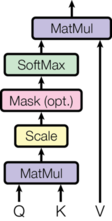
\includegraphics[width=0.2\textwidth]{img/n3.png} 
\caption{Scaled Dot-Product Attention}
\label{Test}
\end{figure}

\begin{equation}
\operatorname{Attention}(Q, K, V)=\operatorname{softmax}\left(\frac{Q K^{T}}{\sqrt{d_{k}}}\right) V
\end{equation}

\begin{Verbatim}
def attention(query, key, value, mask=None, dropout=None):
    "Compute 'Scaled Dot Product Attention'"
    d_k = query.size(-1)
    scores = torch.matmul(query, key.transpose(-2, -1)) \
             / math.sqrt(d_k)
    if mask is not None:
        scores = scores.masked_fill(mask == 0, -1e9)
    p_attn = F.softmax(scores, dim = -1)
    if dropout is not None:
        p_attn = dropout(p_attn)
    return torch.matmul(p_attn, value), p_attn
\end{Verbatim}

两种最常用的Attention函数是加和Attention\footnote{https://arxiv.org/abs/1409.0473}和点积(乘积)Attention,我们的算法与点积 Attention 很类似,但是 $\frac{1}{\sqrt{d_k}}$ 的比例因子不同。加和 Attention 使用具有单个隐藏层的前馈网络来计算兼容函数。虽然两种方法理论上的复杂度是相似的,但在实践中,点积Attention的运算会更快一些,也更节省空间,因为它可以使用高效的矩阵乘法算法来实现。

虽然对于较小的 $d_k$ , 这两种机制的表现相似,但在不放缩较大的 $d_k$ 时,加和 Attention 要优于点 积 Attention\footnote{https://arxiv.org/abs/1703.03906}。我们怀疑,对于较大的 $d_k$,点积大幅增大, 将 Softmax 函数推向具有极小梯度 的区域(为了阐明点积变大的原因,假设 $q$ 和 $k$ 是独立的随机变量, 平均值为 $0$,方差为 $1$,这样他们的点积为 $q \cdot k=\sum_{i=1}^{d_{k}} q_{i} k_{i}$,同样是均值 $0$ 为方差为 $d_k$。为了抵消这种影响,我们用 $\frac{1}{\sqrt{d_k}}$ 来缩放点积。

\begin{figure}[htb]
\centering 
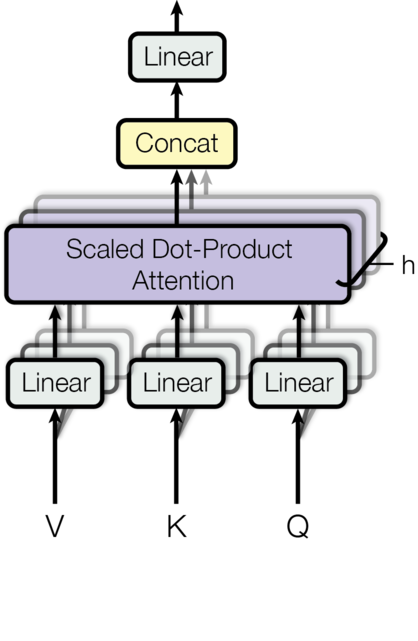
\includegraphics[width=0.4\textwidth]{img/n4.png} 
\caption{Attention}
\label{Test}
\end{figure}

“多头”机制能让模型考虑到不同位置的Attention,另外“多头”Attention 可以在不同的子空间表示不一样的关联关系,使用单个 Head 的 Attention 一般达不到这种效果。

$$\operatorname{MultiHead}(Q, K, V) \&=\operatorname{Concat}\left(\text { head }_{1}, \ldots, \text { head }_{\mathrm{h}}\right) W^{O} $$
\begin{equation}
\text {head}_{\mathrm{i}} \&=\operatorname{Attention}\left(Q W_{i}^{Q}, K W_{i}^{K}, V W_{i}^{V}\right)
\end{equation}

其中参数矩阵为 $W_{i}^{Q} \in \mathbb{R}^{d_{\text {model }} \times d_{k}}, W_{i}^{K} \in \mathbb{R}^{d_{\text {model }} \times d_{k}}, W_{i}^{V} \in \mathbb{R}^{d_{\text {model }} \times d_{v}}$ and $W^{O} \in \mathbb{R}^{h d_{v} \times d_{\text {model }}}$。

我们的工作中使用 $h = 8$ 个 Head 并行的 Attention,对每一个 Head 来说有 $d_{k} = d_{v} = d_{model}/h = 64$ 总计算量与完整维度的单个 Head 的 Attention 很相近。

\begin{Verbatim}
class MultiHeadedAttention(nn.Module):
    def __init__(self, h, d_model, dropout=0.1):
        "Take in model size and number of heads."
        super(MultiHeadedAttention, self).__init__()
        assert d_model % h == 0
        # We assume d_v always equals d_k
        self.d_k = d_model // h
        self.h = h
        self.linears = clones(nn.Linear(d_model, d_model), 4)
        self.attn = None
        self.dropout = nn.Dropout(p=dropout)
        
    def forward(self, query, key, value, mask=None):
        "Implements Figure 2"
        if mask is not None:
            # Same mask applied to all h heads.
            mask = mask.unsqueeze(1)
        nbatches = query.size(0)
        
        # 1) Do all the linear projections in batch from d_model => h x d_k 
        query, key, value = \
            [l(x).view(nbatches, -1, self.h, self.d_k).transpose(1, 2)
             for l, x in zip(self.linears, (query, key, value))]
        
        # 2) Apply attention on all the projected vectors in batch. 
        x, self.attn = attention(query, key, value, mask=mask, 
                                 dropout=self.dropout)
        
        # 3) "Concat" using a view and apply a final linear. 
        x = x.transpose(1, 2).contiguous() \
             .view(nbatches, -1, self.h * self.d_k)
        return self.linears[-1](x)
\end{Verbatim}

7. Attention 在模型中的应用 (Applications of Attention in our Model)

Transformer 中以三种不同的方式使用了 “多头” Attention:

1) 在"Encoder-Decoder Attention"层,Query 来自先前的解码器层,并且 Key 和 Value 来自 Encoder 的输出。Decoder 中的每个位置 Attend 输入序列中的所有位置,这与 Seq2Seq 模型中的经典的 Encoder-Decoder Attention 机制\footnote{https://arxiv.org/abs/1609.08144}一致。

2) Encoder 中的 Self-attention 层。在 Self-attention 层中,所有的 Key、Value 和 Query 都来同一个地方,这里都是来自 Encoder 中前一层的输出。Encoder中当前层的每个位置都能 Attend 到前一层的所有位置。

3) 类似的,解码器中的 Self-attention 层允许解码器中的每个位置 Attend 当前解码位置和它前面的所有位置。这里需要屏蔽解码器中向左的信息流以保持自回归属性。具体的实现方式是在缩放后的点积 Attention 中,屏蔽(设为负无穷)Softmax 的输入中所有对应着非法连接的 Value。

8. Position-wise 前馈网络 (Position-wise Feed-Forward Networks)

除了 Attention 子层之外,Encoder 和 Decoder 中的每个层都包含一个全连接前馈网络,分别地应用于每个位置。其中包括两个线性变换,然后使用 ReLU 作为激活函数。

\begin{equation}
\mathrm{FFN}(x)=\max \left(0, x W_{1}+b_{1}\right) W_{2}+b_{2}
\end{equation}

虽然线性变换在不同位置上是相同的,但它们在层与层之间使用不同的参数。这其实是相当于使用了两个内核大小为 1 的卷积。这里设置输入和输出的维数为 $d_{model} = 512$,内层的维度为 $d_{ff} = 2048$。

\begin{Verbatim}
class PositionwiseFeedForward(nn.Module):
    "Implements FFN equation."
    def __init__(self, d_model, d_ff, dropout=0.1):
        super(PositionwiseFeedForward, self).__init__()
        self.w_1 = nn.Linear(d_model, d_ff)
        self.w_2 = nn.Linear(d_ff, d_model)
        self.dropout = nn.Dropout(dropout)

    def forward(self, x):
        return self.w_2(self.dropout(F.relu(self.w_1(x))))
\end{Verbatim}

9. Embedding 和 Softmax (Embeddings and Softmax)

与其他序列转换模型类似,我们使用预学习的 Embedding 将输入 Token 序列和输出 Token 序列转化为 $d_{model}$ 维向量。我们还使用常用的预训练的线性变换和 Softmax 函数将解码器输出转换为预测下一个 Token 的概率。在我们的模型中,我们在两个 Embedding 层和 Pre-softmax 线性变换之间共享相同的权重矩阵,类似于\footnote{https://arxiv.org/abs/1608.05859}。在 Embedding 层中,我们将这些权重乘以 $\sqrt{d_{model}}$。

\begin{Verbatim}
class Embeddings(nn.Module):
    def __init__(self, d_model, vocab):
        super(Embeddings, self).__init__()
        self.lut = nn.Embedding(vocab, d_model)
        self.d_model = d_model

    def forward(self, x):
        return self.lut(x) * math.sqrt(self.d_model)
\end{Verbatim}

10. 位置编码 (Positional Encoding)

由于我们的模型不包含递归和卷积结构,为了使模型能够有效利用序列的顺序特征,我们需要加入序列中各个Token间相对位置或 Token 在序列中绝对位置的信息。在这里,我们将位置编码添加到编码器和解码器栈底部的输入Embedding。由于位置编码与 Embedding 具有相同的维度$d_{model}$,因此两者可以直接相加。其实这里还有许多位置编码可供选择,其中包括可更新的和固定不变的 \footnote{https://arxiv.org/pdf/1705.03122.pdf}。

在此项工作中,我们使用不同频率的正弦和余弦函数:

\begin{equation}
\begin{aligned}
P E_{(p o s, 2 i)} &=\sin \left(\operatorname{pos} / 10000^{2 i / d_{\text {model }}}\right) \\
P E_{(p o s, 2 i+1)} &=\cos \left(\operatorname{pos} / 10000^{2 i / d_{\text {model }}}\right)
\end{aligned}
\end{equation}

其中 pos 是位置, i 是维度。也就是说,位置编码的每个维度都对应于一个正弦曲线, 其波长形成从 $2\pi$ 到 $10000 \cdot 2 \pi$的等比级数。我们之所以选择了这个函数,是因为我们假设它能让模型很容易学会Attend相对位置, 因为对于任何固定的偏移量 $k$, $PE_{pos+k}$ 可以表示为 $PE_{pos}$ 的线性函数。

此外,在编码器和解码器堆栈中,我们在 Embedding 与位置编码的加和上都使用了 Dropout 机制。 在基本模型上, 我们使用 $PE_{drop} = 0.1$ 的比率。

\begin{Verbatim}
class PositionalEncoding(nn.Module):
    "Implement the PE function."
    def __init__(self, d_model, dropout, max_len=5000):
        super(PositionalEncoding, self).__init__()
        self.dropout = nn.Dropout(p=dropout)
        
        # Compute the positional encodings once in log space.
        pe = torch.zeros(max_len, d_model)
        position = torch.arange(0, max_len).unsqueeze(1)
        div_term = torch.exp(torch.arange(0, d_model, 2) *
                             -(math.log(10000.0) / d_model))
        pe[:, 0::2] = torch.sin(position * div_term)
        pe[:, 1::2] = torch.cos(position * div_term)
        pe = pe.unsqueeze(0)
        self.register_buffer('pe', pe)
        
    def forward(self, x):
        x = x + Variable(self.pe[:, :x.size(1)], 
                         requires_grad=False)
        return self.dropout(x)
\end{Verbatim}

如下所示,位置编码将根据位置添加正弦曲线。曲线的频率和偏移对于每个维度是不同的。

\begin{Verbatim}
plt.figure(figsize=(15, 5))
pe = PositionalEncoding(20, 0)
y = pe.forward(Variable(torch.zeros(1, 100, 20)))
plt.plot(np.arange(100), y[0, :, 4:8].data.numpy())
plt.legend(["dim %d"%p for p in [4,5,6,7]])
None
\end{Verbatim}

\begin{figure}[htb]
\centering 
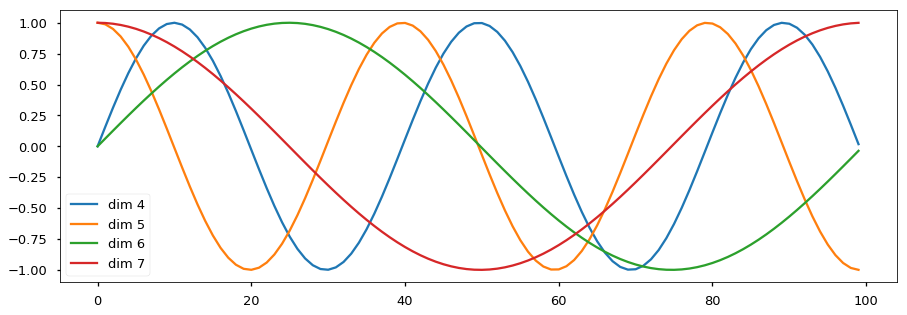
\includegraphics[width=0.8\textwidth]{img/n5.png} 
\caption{曲线的频率和偏移}
\label{Test}
\end{figure}

11. 完整模型 (Full Model)

下面定义了连接完整模型并设置超参的函数。

\begin{Verbatim}
def make_model(src_vocab, tgt_vocab, N=6, 
               d_model=512, d_ff=2048, h=8, dropout=0.1):
    "Helper: Construct a model from hyperparameters."
    c = copy.deepcopy
    attn = MultiHeadedAttention(h, d_model)
    ff = PositionwiseFeedForward(d_model, d_ff, dropout)
    position = PositionalEncoding(d_model, dropout)
    model = EncoderDecoder(
        Encoder(EncoderLayer(d_model, c(attn), c(ff), dropout), N),
        Decoder(DecoderLayer(d_model, c(attn), c(attn), 
                             c(ff), dropout), N),
        nn.Sequential(Embeddings(d_model, src_vocab), c(position)),
        nn.Sequential(Embeddings(d_model, tgt_vocab), c(position)),
        Generator(d_model, tgt_vocab))
    
    # This was important from their code. 
    # Initialize parameters with Glorot / fan_avg.
    for p in model.parameters():
        if p.dim() > 1:
            #nn.init.xavier_uniform(p)
            nn.init.xavier_uniform_(p)
    return model
\end{Verbatim}

\begin{Verbatim}
# Small example model.
tmp_model = make_model(10, 10, 2)
None
\end{Verbatim}

12. 训练 (Training)

本节介绍模型的训练方法。

快速穿插介绍训练标准编码器解码器模型需要的一些工具。首先我们定义一个包含源和目标句子的批训练对象用于训练,同时构造掩码。

13. 批和掩码 (Batches and Masking)

\begin{Verbatim}
class Batch:
    "Object for holding a batch of data with mask during training."
    def __init__(self, src, trg=None, pad=0):
        self.src = src
        self.src_mask = (src != pad).unsqueeze(-2)
        if trg is not None:
            self.trg = trg[:, :-1]
            self.trg_y = trg[:, 1:]
            self.trg_mask = \
                self.make_std_mask(self.trg, pad)
            self.ntokens = (self.trg_y != pad).data.sum()
    
    @staticmethod
    def make_std_mask(tgt, pad):
        "Create a mask to hide padding and future words."
        tgt_mask = (tgt != pad).unsqueeze(-2)
        tgt_mask = tgt_mask & Variable(
            subsequent_mask(tgt.size(-1)).type_as(tgt_mask.data))
        return tgt_mask
\end{Verbatim}

接下来,我们创建一个通用的训练和得分函数来跟踪损失。我们传入一个通用的损失计算函数,它也处理参数更新。

14. 训练循环 (Training Loop)

\begin{Verbatim}
def run_epoch(data_iter, model, loss_compute):
    "Standard Training and Logging Function"
    start = time.time()
    total_tokens = 0
    total_loss = 0
    tokens = 0
    for i, batch in enumerate(data_iter):
        out = model.forward(batch.src, batch.trg, 
                            batch.src_mask, batch.trg_mask)
        loss = loss_compute(out, batch.trg_y, batch.ntokens)
        total_loss += loss
        total_tokens += batch.ntokens
        tokens += batch.ntokens
        if i % 50 == 1:
            elapsed = time.time() - start
            print("Epoch Step: %d Loss: %f Tokens per Sec: %f" %
                    (i, loss / batch.ntokens, tokens / elapsed))
            start = time.time()
            tokens = 0
    return total_loss / total_tokens
\end{Verbatim}

15. 训练数据和批处理 (Training Data and Batching)

我们使用标准 WMT 2014 英语-德语数据集进行了训练,该数据集包含大约 450 万个句子对。 使用字节对的编码方法对句子进行编码,该编码具有大约37000个词的共享源-目标词汇表。 对于英语-法语,我们使用了 WMT 2014 英语-法语数据集,该数据集由36M个句子组成,并将词分成32000个词片(Word-piece)的词汇表。

句子对按照近似的序列长度进行批处理。每个训练批包含一组句子对,包含大约 25000 个源词和 25000 个目标词。

我们将使用torch text来创建批次。下面更详细地讨论实现过程。 我们在torchtext的一个函数中创建批次,确保填充到最大批训练长度的大小不超过阈值(如果我们有8个GPU,则阈值为 25000)。

\begin{Verbatim}
global max_src_in_batch, max_tgt_in_batch
def batch_size_fn(new, count, sofar):
    "Keep augmenting batch and calculate total number of tokens + padding."
    global max_src_in_batch, max_tgt_in_batch
    if count == 1:
        max_src_in_batch = 0
        max_tgt_in_batch = 0
    max_src_in_batch = max(max_src_in_batch,  len(new.src))
    max_tgt_in_batch = max(max_tgt_in_batch,  len(new.trg) + 2)
    src_elements = count * max_src_in_batch
    tgt_elements = count * max_tgt_in_batch
    return max(src_elements, tgt_elements)
\end{Verbatim}

16. 硬件和训练进度 (Hardware and Schedule)

我们在一台配备8个NVIDIA P100 GPU的机器上训练我们的模型。 对于使用本文所述的超参数的基本模型,每个训练单步大约需要0.4秒。 我们对基础模型进行了总共100,000步或12小时的训练。 对于我们的大型模型,每个训练单步时间为1.0秒。 大型模型通常需要训练300,000步(3.5天)。

17. 优化器 (Optimizer)

我们选择Adam \footnote{https://arxiv.org/abs/1412.6980}作为优化器,其参数为 $\beta_{1}=0.9, \beta_{2}=0.98$ 和 $\epsilon=10^{-9}$. 根据以下公式,我们在训练过程中改变了学习率:

\begin{equation}
\text { lrate }=d_{\text {model }}^{-0.5} \cdot \min \left(\text { step\_num }^{-0.5}, \text { step\_num } \cdot \text { warmup\_steps }^{-1.5}\right)
\end{equation}

在预热中随步数线性地增加学习速率,并且此后与步数的反平方根成比例地减小它。我们设置预热步数为 4000。

注意:这部分非常重要,需要这种设置训练模型。

\begin{Verbatim}
class NoamOpt:
    "Optim wrapper that implements rate."
    def __init__(self, model_size, factor, warmup, optimizer):
        self.optimizer = optimizer
        self._step = 0
        self.warmup = warmup
        self.factor = factor
        self.model_size = model_size
        self._rate = 0
        
    def step(self):
        "Update parameters and rate"
        self._step += 1
        rate = self.rate()
        for p in self.optimizer.param_groups:
            p['lr'] = rate
        self._rate = rate
        self.optimizer.step()
        
    def rate(self, step = None):
        "Implement `lrate` above"
        if step is None:
            step = self._step
        return self.factor * \
            (self.model_size ** (-0.5) *
            min(step ** (-0.5), step * self.warmup ** (-1.5)))
        
def get_std_opt(model):
    return NoamOpt(model.src_embed[0].d_model, 2, 4000,
            torch.optim.Adam(model.parameters(), lr=0, betas=(0.9, 0.98), eps=1e-9))
\end{Verbatim}

当前模型在不同模型大小和超参数的情况下的曲线示例。

\begin{Verbatim}
# Three settings of the lrate hyperparameters.
opts = [NoamOpt(512, 1, 4000, None), 
        NoamOpt(512, 1, 8000, None),
        NoamOpt(256, 1, 4000, None)]
plt.plot(np.arange(1, 20000), [[opt.rate(i) for opt in opts] for i in range(1, 20000)])
plt.legend(["512:4000", "512:8000", "256:4000"])
None
\end{Verbatim}

\begin{figure}[htb]
\centering 
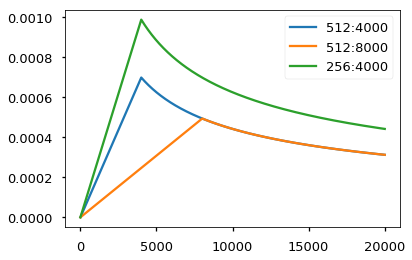
\includegraphics[width=0.65\textwidth]{img/n6.png} 
\caption{当前模型在不同模型大小和超参数的情况下的曲线示例}
\label{Test}
\end{figure}

18. 正则化 (Regularization)

19. 标签平滑 (Label Smoothing)

在训练期间,我们采用了值 $\epsilon_{l s}=0.1$ \footnote{https://arxiv.org/abs/1512.00567}的标签平滑。 这种做法提高了困惑度,因为模型变得更加不确定,但提高了准确性和BLEU分数。

我们使用 KL div loss 实现标签平滑。 相比使用独热目标分布,我们创建一个分布,其包含正确单词的置信度和整个词汇表中分布的其余平滑项。

\begin{Verbatim}
class LabelSmoothing(nn.Module):
    "Implement label smoothing."
    def __init__(self, size, padding_idx, smoothing=0.0):
        super(LabelSmoothing, self).__init__()
        #self.criterion = nn.KLDivLoss(size_average=False)reduction='sum’
        self.criterion = nn.KLDivLoss(reduction='sum')
        self.padding_idx = padding_idx
        self.confidence = 1.0 - smoothing
        self.smoothing = smoothing
        self.size = size
        self.true_dist = None
        
    def forward(self, x, target):
        assert x.size(1) == self.size
        true_dist = x.data.clone()
        true_dist.fill_(self.smoothing / (self.size - 2))
        true_dist.scatter_(1, target.data.unsqueeze(1), self.confidence)
        true_dist[:, self.padding_idx] = 0
        mask = torch.nonzero(target.data == self.padding_idx)
        if mask.dim() > 0:
            true_dist.index_fill_(0, mask.squeeze(), 0.0)
        self.true_dist = true_dist
        return self.criterion(x, Variable(true_dist, requires_grad=False))
\end{Verbatim}

在这里,我们可以看到标签平滑的示例。

\begin{Verbatim}
# Example of label smoothing.
crit = LabelSmoothing(5, 0, 0.4)
predict = torch.FloatTensor([[0, 0.2, 0.7, 0.1, 0],
                             [0, 0.2, 0.7, 0.1, 0], 
                             [0, 0.2, 0.7, 0.1, 0]])
v = crit(Variable(predict.log()), 
         Variable(torch.LongTensor([2, 1, 0])))

# Show the target distributions expected by the system.
plt.imshow(crit.true_dist)
None
\end{Verbatim}

\begin{figure}[htb]
\centering 
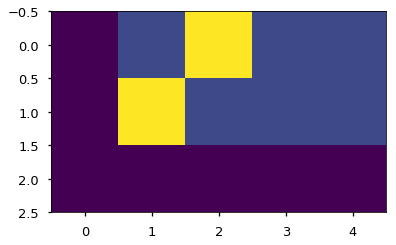
\includegraphics[width=0.5\textwidth]{img/n7.png} 
\caption{标签平滑的示例}
\label{Test}
\end{figure}

如果对给定的选择非常有信心,标签平滑实际上会开始惩罚模型。

\begin{Verbatim}
crit = LabelSmoothing(5, 0, 0.1)
def loss(x):
    d = x + 3 * 1
    predict = torch.FloatTensor([[0, x / d, 1 / d, 1 / d, 1 / d],])
    #print(predict)
    #return crit(Variable(predict.log()), Variable(torch.LongTensor([1]))).data[0]
    return crit(Variable(predict.log()), Variable(torch.LongTensor([1]))).item()
plt.plot(np.arange(1, 100), [loss(x) for x in range(1, 100)])
None
\end{Verbatim}

\begin{figure}[htb]
\centering 
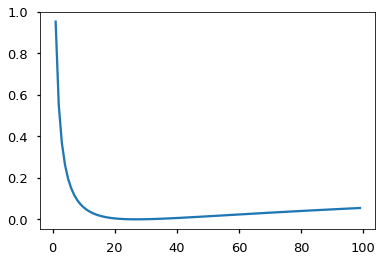
\includegraphics[width=0.6\textwidth]{img/n8.png} 
\caption{标签平滑实际上会开始惩罚模型}
\label{Test}
\end{figure}

20. 第一个例子 (A First Example)

我们可以先尝试一个简单的复制任务。 给定来自小词汇表的随机输入符号集,目标是生成那些相同的符号。

21. 数据生成 (Synthetic Data)

\begin{Verbatim}
def data_gen(V, batch, nbatches):
    "Generate random data for a src-tgt copy task."
    for i in range(nbatches):
        data = torch.from_numpy(np.random.randint(1, V, size=(batch, 10)))
        data[:, 0] = 1
        src = Variable(data, requires_grad=False)
        tgt = Variable(data, requires_grad=False)
        yield Batch(src, tgt, 0)
\end{Verbatim}

22. 损失计算 (Loss Computation)

\begin{Verbatim}
class SimpleLossCompute:
    "A simple loss compute and train function."
    def __init__(self, generator, criterion, opt=None):
        self.generator = generator
        self.criterion = criterion
        self.opt = opt
        
    def __call__(self, x, y, norm):
        x = self.generator(x)
        loss = self.criterion(x.contiguous().view(-1, x.size(-1)), 
                              y.contiguous().view(-1)) / norm
        loss.backward()
        if self.opt is not None:
            self.opt.step()
            self.opt.optimizer.zero_grad()
        #return loss.data[0] * norm
        return loss.item() * norm
    #.item()
\end{Verbatim}

23. 贪心解码 (Greedy Decoding)

\begin{Verbatim}
# Train the simple copy task.
V = 11
criterion = LabelSmoothing(size=V, padding_idx=0, smoothing=0.0)
model = make_model(V, V, N=2)
model_opt = NoamOpt(model.src_embed[0].d_model, 1, 400,
        torch.optim.Adam(model.parameters(), lr=0, betas=(0.9, 0.98), eps=1e-9))

for epoch in range(10):
    model.train()
    run_epoch(data_gen(V, 30, 20), model, SimpleLossCompute(model.generator, criterion, model_opt))
    model.eval()
    print(run_epoch(data_gen(V, 30, 5), model, 
                    SimpleLossCompute(model.generator, criterion, None)))
\end{Verbatim}

该作业实际输出如下 :

\begin{Verbatim}
Epoch Step: 1 Loss: 2.952445 Tokens per Sec: 576.319092
Epoch Step: 1 Loss: 1.998418 Tokens per Sec: 698.345398
tensor(1.9607)
Epoch Step: 1 Loss: 1.944340 Tokens per Sec: 607.740173
Epoch Step: 1 Loss: 1.703401 Tokens per Sec: 697.352722
tensor(1.6663)
Epoch Step: 1 Loss: 1.836476 Tokens per Sec: 608.583740
Epoch Step: 1 Loss: 1.518878 Tokens per Sec: 698.963074
tensor(1.4429)
Epoch Step: 1 Loss: 1.751896 Tokens per Sec: 611.272522
Epoch Step: 1 Loss: 1.445300 Tokens per Sec: 699.340576
tensor(1.4257)
Epoch Step: 1 Loss: 1.457413 Tokens per Sec: 609.735352
Epoch Step: 1 Loss: 0.952619 Tokens per Sec: 700.159241
tensor(0.9635)
Epoch Step: 1 Loss: 1.194762 Tokens per Sec: 603.452271
Epoch Step: 1 Loss: 0.720170 Tokens per Sec: 699.754761
tensor(0.6950)
Epoch Step: 1 Loss: 1.114729 Tokens per Sec: 610.193848
Epoch Step: 1 Loss: 0.482503 Tokens per Sec: 694.832153
tensor(0.4766)
Epoch Step: 1 Loss: 0.910544 Tokens per Sec: 605.345947
Epoch Step: 1 Loss: 0.245647 Tokens per Sec: 699.077209
tensor(0.3241)
Epoch Step: 1 Loss: 0.579662 Tokens per Sec: 606.469055
Epoch Step: 1 Loss: 0.210620 Tokens per Sec: 678.093811
tensor(0.2678)
Epoch Step: 1 Loss: 0.556862 Tokens per Sec: 575.055847
Epoch Step: 1 Loss: 0.189768 Tokens per Sec: 690.105469
tensor(0.2050)
\end{Verbatim}

为简单起见,此代码使用贪心解码来预测翻译。

\begin{Verbatim}
def greedy_decode(model, src, src_mask, max_len, start_symbol):
    memory = model.encode(src, src_mask)
    ys = torch.ones(1, 1).fill_(start_symbol).type_as(src.data)
    for i in range(max_len-1):
        out = model.decode(memory, src_mask, 
                           Variable(ys), 
                           Variable(subsequent_mask(ys.size(1))
                                    .type_as(src.data)))
        prob = model.generator(out[:, -1])
        _, next_word = torch.max(prob, dim = 1)
        #next_word = next_word.data[0]
        next_word = next_word.item()
        ys = torch.cat([ys, 
                        torch.ones(1, 1).type_as(src.data).fill_(next_word)], dim=1)
    return ys

model.eval()
src = Variable(torch.LongTensor([[1,2,3,4,5,6,7,8,9,10]]) )
src_mask = Variable(torch.ones(1, 1, 10) )
print(greedy_decode(model, src, src_mask, max_len=10, start_symbol=1))
\end{Verbatim}

24. 真实示例 (A Real World Example)

现在我们通过IWSLT德语-英语翻译任务介绍一个真实示例。 该任务比上文提及的WMT任务小得多,但它说明了整个系统。 我们还展示了如何使用多个 GPU 处理加速其训练。

本作业至第 24 节 真实示例 (A Real World Example)后,因为套件与本版本错误,选择用注解说明。

\begin{Verbatim}
#!pip install torchtext spacy
#!python -m spacy download en
#!python -m spacy download de
\end{Verbatim}

25. 数据加载 (Data Loading)

我们将使用torchtext和spacy加载数据集以进行词语切分。

\begin{Verbatim}
# For data loading.
from torchtext import data, datasets

if True:
    import spacy
    spacy_de = spacy.load('de')
    spacy_en = spacy.load('en')

    def tokenize_de(text):
        return [tok.text for tok in spacy_de.tokenizer(text)]

    def tokenize_en(text):
        return [tok.text for tok in spacy_en.tokenizer(text)]

    BOS_WORD = '<s>'
    EOS_WORD = '</s>'
    BLANK_WORD = "<blank>"
    SRC = data.Field(tokenize=tokenize_de, pad_token=BLANK_WORD)
    TGT = data.Field(tokenize=tokenize_en, init_token = BOS_WORD, 
                     eos_token = EOS_WORD, pad_token=BLANK_WORD)

    MAX_LEN = 100
    train, val, test = datasets.IWSLT.splits(
        exts=('.de', '.en'), fields=(SRC, TGT), 
        filter_pred=lambda x: len(vars(x)['src']) <= MAX_LEN and 
            len(vars(x)['trg']) <= MAX_LEN)
    MIN_FREQ = 2
    SRC.build_vocab(train.src, min_freq=MIN_FREQ)
    TGT.build_vocab(train.trg, min_freq=MIN_FREQ)
\end{Verbatim}

批训练对于速度来说很重要。我们希望批次分割非常均匀并且填充最少。 要做到这一点,我们必须修改torchtext默认的批处理函数。 这部分代码修补其默认批处理函数,以确保我们搜索足够多的句子以构建紧密批处理。

26. 迭代器 (Iterators)

\begin{Verbatim}
class MyIterator(data.Iterator):
    def create_batches(self):
        if self.train:
            def pool(d, random_shuffler):
                for p in data.batch(d, self.batch_size * 100):
                    p_batch = data.batch(
                        sorted(p, key=self.sort_key),
                        self.batch_size, self.batch_size_fn)
                    for b in random_shuffler(list(p_batch)):
                        yield b
            self.batches = pool(self.data(), self.random_shuffler)
            
        else:
            self.batches = []
            for b in data.batch(self.data(), self.batch_size,
                                          self.batch_size_fn):
                self.batches.append(sorted(b, key=self.sort_key))

def rebatch(pad_idx, batch):
    "Fix order in torchtext to match ours"
    src, trg = batch.src.transpose(0, 1), batch.trg.transpose(0, 1)
    return Batch(src, trg, pad_idx)
\end{Verbatim}

27. 多 GPU 训练 (Multi-GPU Training)

最后为了真正地快速训练,我们将使用多个GPU。 这部分代码实现了多GPU字生成。 它不是Transformer特有的,所以我不会详细介绍。 其思想是将训练时的单词生成分成块,以便在许多不同的GPU上并行处理。 我们使用PyTorch并行原语来做到这一点:

\begin{itemize}
\item [-] 复制 - 将模块拆分到不同的 GPU 上
\item [-] 分散 - 将批次拆分到不同的 GPU 上
\item [-] 并行应用 - 在不同 GPU 上将模块应用于批处理
\item [-] 聚集 - 将分散的数据聚集到一个 GPU 上
\item [-] nn.DataParallel - 一个特殊的模块包装器,在评估之前调用它们。
\end{itemize}

\begin{Verbatim}
# Skip if not interested in multigpu.
class MultiGPULossCompute:
    "A multi-gpu loss compute and train function."
    def __init__(self, generator, criterion, devices, opt=None, chunk_size=5):
        # Send out to different gpus.
        self.generator = generator
        self.criterion = nn.parallel.replicate(criterion, 
                                               devices=devices)
        self.opt = opt
        self.devices = devices
        self.chunk_size = chunk_size
        
    def __call__(self, out, targets, normalize):
        total = 0.0
        generator = nn.parallel.replicate(self.generator, 
                                                devices=self.devices)
        out_scatter = nn.parallel.scatter(out, 
                                          target_gpus=self.devices)
        out_grad = [[] for _ in out_scatter]
        targets = nn.parallel.scatter(targets, 
                                      target_gpus=self.devices)

        # Divide generating into chunks.
        chunk_size = self.chunk_size
        for i in range(0, out_scatter[0].size(1), chunk_size):
            # Predict distributions
            out_column = [[Variable(o[:, i:i+chunk_size].data, 
                                    requires_grad=self.opt is not None)] 
                           for o in out_scatter]
            gen = nn.parallel.parallel_apply(generator, out_column)

            # Compute loss. 
            y = [(g.contiguous().view(-1, g.size(-1)), 
                  t[:, i:i+chunk_size].contiguous().view(-1)) 
                 for g, t in zip(gen, targets)]
            loss = nn.parallel.parallel_apply(self.criterion, y)

            # Sum and normalize loss
            l = nn.parallel.gather(loss, 
                                   target_device=self.devices[0])
            l = l.sum()[0] / normalize
            total += l.data[0]

            # Backprop loss to output of transformer
            if self.opt is not None:
                l.backward()
                for j, l in enumerate(loss):
                    out_grad[j].append(out_column[j][0].grad.data.clone())

        # Backprop all loss through transformer.            
        if self.opt is not None:
            out_grad = [Variable(torch.cat(og, dim=1)) for og in out_grad]
            o1 = out
            o2 = nn.parallel.gather(out_grad, 
                                    target_device=self.devices[0])
            o1.backward(gradient=o2)
            self.opt.step()
            self.opt.optimizer.zero_grad()
        return total * normalize
\end{Verbatim}

现在我们创建模型,损失函数,优化器,数据迭代器和并行化。

\begin{Verbatim}
# GPUs to use
devices = [0, 1, 2, 3]
if True:
    pad_idx = TGT.vocab.stoi["<blank>"]
    model = make_model(len(SRC.vocab), len(TGT.vocab), N=6)
    model.cuda()
    criterion = LabelSmoothing(size=len(TGT.vocab), padding_idx=pad_idx, smoothing=0.1)
    criterion.cuda()
    BATCH_SIZE = 12000
    train_iter = MyIterator(train, batch_size=BATCH_SIZE, device=0,
                            repeat=False, sort_key=lambda x: (len(x.src), len(x.trg)),
                            batch_size_fn=batch_size_fn, train=True)
    valid_iter = MyIterator(val, batch_size=BATCH_SIZE, device=0,
                            repeat=False, sort_key=lambda x: (len(x.src), len(x.trg)),
                            batch_size_fn=batch_size_fn, train=False)
    model_par = nn.DataParallel(model, device_ids=devices)
None
\end{Verbatim}

现在我们训练模型。 我将稍微使用预热步骤,但其他一切都使用默认参数。 在具有4个Tesla V100 GPU的AWS p3.8xlarge机器上,每秒运行约27,000个词,批训练大小大小为12,000。

28. 训练系统 (Training the System)

\begin{Verbatim}
#!wget https://s3.amazonaws.com/opennmt-models/iwslt.pt

if False:
    model_opt = NoamOpt(model.src_embed[0].d_model, 1, 2000,
            torch.optim.Adam(model.parameters(), lr=0, betas=(0.9, 0.98), eps=1e-9))
    for epoch in range(10):
        model_par.train()
        run_epoch((rebatch(pad_idx, b) for b in train_iter), 
                  model_par, 
                  MultiGPULossCompute(model.generator, criterion, 
                                      devices=devices, opt=model_opt))
        model_par.eval()
        loss = run_epoch((rebatch(pad_idx, b) for b in valid_iter), 
                          model_par, 
                          MultiGPULossCompute(model.generator, criterion, 
                          devices=devices, opt=None))
        print(loss)
else:
    model = torch.load("iwslt.pt")
\end{Verbatim}

一旦训练完成,我们可以解码模型以产生一组翻译。 在这里,我们只需翻译验证集中的第一个句子。 此数据集非常小,因此使用贪婪搜索的翻译相当准确。

\begin{Verbatim}
for i, batch in enumerate(valid_iter):
    src = batch.src.transpose(0, 1)[:1]
    src_mask = (src != SRC.vocab.stoi["<blank>"]).unsqueeze(-2)
    out = greedy_decode(model, src, src_mask, 
                        max_len=60, start_symbol=TGT.vocab.stoi["<s>"])
    print("Translation:", end="\t")
    for i in range(1, out.size(1)):
        sym = TGT.vocab.itos[out[0, i]]
        if sym == "</s>": break
        print(sym, end =" ")
    print()
    print("Target:", end="\t")
    for i in range(1, batch.trg.size(0)):
        sym = TGT.vocab.itos[batch.trg.data[i, 0]]
        if sym == "</s>": break
        print(sym, end =" ")
    print()
    break
\end{Verbatim}

29. 附加组件:BPE,搜索,平均 (Additional Components: BPE, Search, Averaging)

所以这主要涵盖了Transformer模型本身。 有四个方面我们没有明确涵盖。 我们还实现了所有这些附加功能 OpenNMT-py.

1) 字节对编码/ 字片(Word-piece):我们可以使用库来首先将数据预处理为子字单元。参见Rico Sennrich的subword-nmt实现。这些模型将训练数据转换为如下所示:

\begin{Verbatim}
▁Die ▁Protokoll datei ▁kann ▁ heimlich ▁per ▁E - Mail 
▁oder ▁FTP ▁an ▁einen ▁bestimmte n ▁Empfänger ▁gesendet ▁werden .
\end{Verbatim}

2) 共享嵌入:当使用具有共享词汇表的BPE时,我们可以在源/目标/生成器之间共享相同的权重向量,详细见。 要将其添加到模型,只需执行以下操作:

\begin{Verbatim}
if False:
    model.src_embed[0].lut.weight = model.tgt_embeddings[0].lut.weight
    model.generator.lut.weight = model.tgt_embed[0].lut.weight
\end{Verbatim}

3) 集束搜索:这里展开说有点太复杂了。 PyTorch 版本的实现可以参考 OpenNMT- py。
4) 模型平均:这篇文章平均最后k个检查点以创建一个集合效果。 如果我们有一堆模型,我们可以在事后这样做:

\begin{Verbatim}
def average(model, models):
    "Average models into model"
    for ps in zip(*[m.params() for m in [model] + models]):
        p[0].copy_(torch.sum(*ps[1:]) / len(ps[1:]))
\end{Verbatim}

30. 结果 (Results)

在 WMT 2014英语-德语翻译任务中,大型 Transformer 模型(表中的Transformer(大))优于先前报告的最佳模型(包括集成的模型)超过2.0 BLEU,建立了一个新的最先进BLEU得分为28.4。 该模型的配置列于表3的底部。在8个P100 GPU的机器上,训练需要需要3.5天。 甚至我们的基础模型也超过了之前发布的所有模型和集成,而且只占培训成本的一小部分。

在WMT 2014英语-法语翻译任务中,我们的大型模型获得了41.0的BLEU分数,优于以前发布的所有单一模型,不到以前最先进技术培训成本的1/4 模型。 使用英语到法语训练的Transformer(大)模型使用dropout概率 $P_{dorp}=0.1$ ,而不是0.3。

\begin{figure}[htb]
\centering 
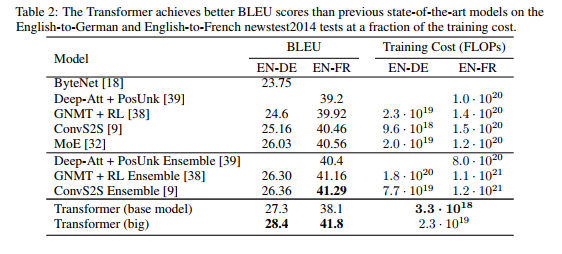
\includegraphics[width=0.9\textwidth]{img/n9.png} 
\caption{WMT 2014英语-德语翻译任}
\label{Test}
\end{figure}

\begin{Verbatim}
!wget https://s3.amazonaws.com/opennmt-models/en-de-model.pt
\end{Verbatim}

\begin{Verbatim}
model, SRC, TGT = torch.load("en-de-model.pt")
\end{Verbatim}

\begin{Verbatim}
model.eval()
sent = "▁The ▁log ▁file ▁can ▁be ▁sent ▁secret ly ▁with ▁email ▁or ▁FTP ▁to ▁a ▁specified ▁receiver".split()
src = torch.LongTensor([[SRC.stoi[w] for w in sent]])
src = Variable(src)
src_mask = (src != SRC.stoi["<blank>"]).unsqueeze(-2)
out = greedy_decode(model, src, src_mask, 
                    max_len=60, start_symbol=TGT.stoi["<s>"])
print("Translation:", end="\t")
trans = "<s> "
for i in range(1, out.size(1)):
    sym = TGT.itos[out[0, i]]
    if sym == "</s>": break
    trans += sym + " "
print(trans)
\end{Verbatim}

31. 注意力可视化 (Attention Visualization)

即使使用贪婪的解码器,翻译看起来也不错。 我们可以进一步想象它,看看每一层注意力发生了什么。

\begin{Verbatim}
tgt_sent = trans.split()
def draw(data, x, y, ax):
    seaborn.heatmap(data, 
                    xticklabels=x, square=True, yticklabels=y, vmin=0.0, vmax=1.0, 
                    cbar=False, ax=ax)
    
for layer in range(1, 6, 2):
    fig, axs = plt.subplots(1,4, figsize=(20, 10))
    print("Encoder Layer", layer+1)
    for h in range(4):
        draw(model.encoder.layers[layer].self_attn.attn[0, h].data, 
            sent, sent if h ==0 else [], ax=axs[h])
    plt.show()
    
for layer in range(1, 6, 2):
    fig, axs = plt.subplots(1,4, figsize=(20, 10))
    print("Decoder Self Layer", layer+1)
    for h in range(4):
        draw(model.decoder.layers[layer].self_attn.attn[0, h].data[:len(tgt_sent), :len(tgt_sent)], 
            tgt_sent, tgt_sent if h ==0 else [], ax=axs[h])
    plt.show()
    print("Decoder Src Layer", layer+1)
    fig, axs = plt.subplots(1,4, figsize=(20, 10))
    for h in range(4):
        draw(model.decoder.layers[layer].self_attn.attn[0, h].data[:len(tgt_sent), :len(sent)], 
            sent, tgt_sent if h ==0 else [], ax=axs[h])
    plt.show()
\end{Verbatim}

32. 结论 (Conclusion)

\begin{Verbatim}
@inproceedings{opennmt,
  author    = {Guillaume Klein and
               Yoon Kim and
               Yuntian Deng and
               Jean Senellart and
               Alexander M. Rush},
  title     = {OpenNMT: Open-Source Toolkit for Neural Machine Translation},
  booktitle = {Proc. ACL},
  year      = {2017},
  url       = {https://doi.org/10.18653/v1/P17-4012},
  doi       = {10.18653/v1/P17-4012}
}
\end{Verbatim}

\subsection{Chatbot Transformer}

该范例为 fawazsammani/chatbot-transformer 的 GitHub 专案,该专案使用 Cornell Movie Dialog Corpus 资料,进行 Chatbot using Transformers 的实作,其训练结果如下。

\begin{figure}[htb]
\centering 
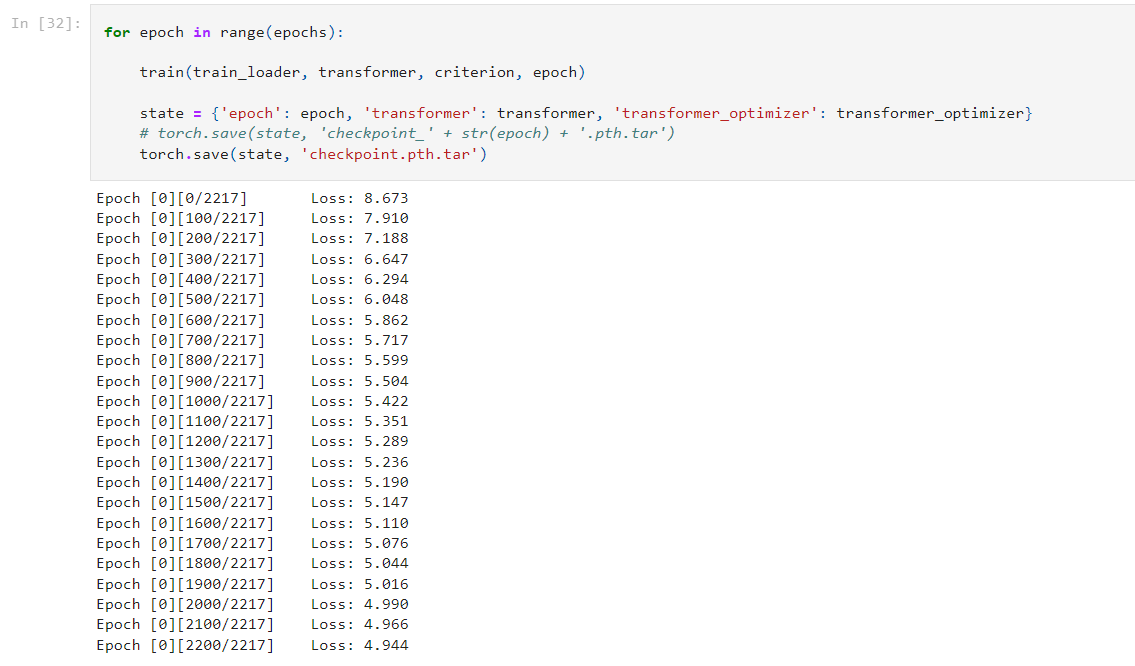
\includegraphics[width=0.95\textwidth]{img/n10.png} 
\caption{Chatbot Transformer 训练}
\label{Test}
\end{figure}

\section{使用技术}

在此次作业有试验过不同的技术实践,比如虚拟化容器的演练。此次作业有尝试演练 Docker 与 LaTeX 来改善研究工作流程。

\subsection{LaTeX}

LaTex 为 Overleaf 的模板,其模板贡献则是根据 iofu728-pkuthss 的版本进行作业。

\subsection{Docker}

在此使用 Anaconda 的 Docker 容器,并用共同挂载目录进行流程。

1. 在终端窗口中,运行此命令以显示可用图像列表:

\begin{Verbatim}
docker search continuumio
\end{Verbatim}

2.拉取所需的图像

\begin{Verbatim}
docker pull continuumio/miniconda3
\end{Verbatim}

3. 使用图像创建容器

\begin{Verbatim}
docker run -t -i continuumio/miniconda3 /bin/bash
\end{Verbatim}

4. 若想在本地挂载目录则用 -v ,假设本机使用 Windows 在目录 docker-save,而 /share 为 Docker 的目录。

\begin{Verbatim}
# docker run -it -v D:\docker-save:/share continuumio/miniconda3 /bin/bash
# docker run -it -v [本地端目录]:[Docker 目录] [Docker 映像的名称] /bin/bash
\end{Verbatim}

5. 安装和启动 Jupyter Notebook

请在浏览器中打开 http://localhost:8888

\begin{Verbatim}
docker run -i -t -p 8888:8888 continuumio/miniconda3 /bin/bash -c "\
    conda install jupyter -y --quiet && \
    mkdir -p /opt/notebooks && \
    jupyter notebook \
    --notebook-dir=/opt/notebooks --ip='*' --port=8888 \
    --no-browser --allow-root"
\end{Verbatim}

6. 根据前述设定好路径,则合理的配置如下。

\begin{Verbatim}
docker run -i -t -v D:\docker-save:/opt/notebooks -p 8888:8888 continuumio/miniconda3 /bin/bash -c "\
    conda install jupyter -y --quiet && \
    mkdir -p /opt/notebooks && \
    jupyter notebook \
    --notebook-dir=/opt/notebooks --ip='*' --port=8888 \
    --no-browser --allow-root"
\end{Verbatim}

7. 管理容器

docker ps 看所有映像档,而 -a 列出包含未运行的

\begin{Verbatim}
docker ps
docker ps -a
\end{Verbatim}
